% background chapter continued
\section{Software Design Principles}
This section mentions few core design principles necessary to maintain healthy codebase and knowledge to
build scalable software. The design patterns are abstract and universally applied in different programming paradigms.
\\
\\
\subsection{Open-Close Principle}
When a certain code is designed with an intent to extend it but does not need any modification
whenever requirements change or when new use-case is requested, such code is said obeying open-close
principle. In other words, it is open for extension and closed modificaiton. This design process gives
more flexibility to the program and make future changes cheaper.

\begin{figure}[h!]
  \centering
  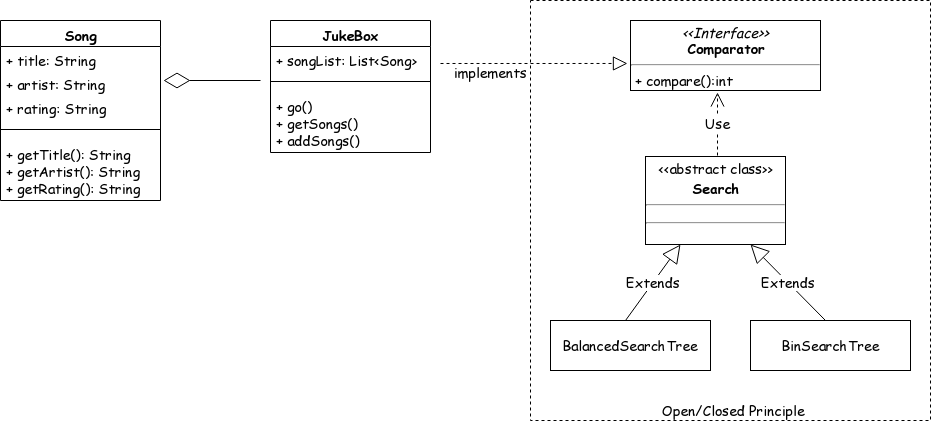
\includegraphics[width=15cm,height=12cm,keepaspectratio]{../media/crawler/opencloseprinciple.png}
  \caption{A example JukeBox program using Open/Close Principle}
  \label{fig:jukebox}
\end{figure}

\noindent
Consider an example of this principle in image \ref{fig:jukebox}, the Jukebox inner class implements Comparator interface, overriding compare method to search on different attributes of the class (eg. search on title, artist, etc). That method is invoked from concrete implementation of abstract Search class.
algorithm upon calling Collections.search(). The search functionality offered by two concrete class vary
independently and their runtime doesn't affect each other. Even more search algorithms can added without
affecting existing search. The same comparators in JukeBox can also be used to perform sorting on songs
called by respective sorting algorithm overriding sort method from sort interface.

\pagebreak

\subsection{Dependency Injection}
Dependency Injection(DI) promotes open-closed principle and reduces loose coupling. It is one of the most
important topics applicable to almost all software produced. DI provides references to objects the class
depends on instead of allowing class to gather dependencies by itself. The dependent class doesn't
take into account the how, where and what of implementation. This makes great impact on the flexibility of
software design.
\begin{figure}[h!]
  \centering
  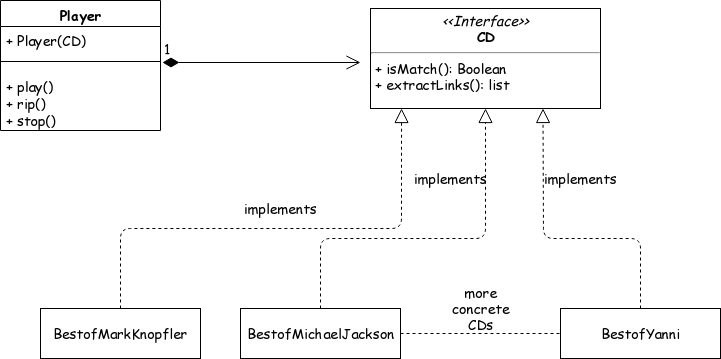
\includegraphics[width=15cm,height=12cm,keepaspectratio]{../media/crawler/dinjection.png}
  \caption{CD Player using Dependency Injection}
  \label{fig:dinjection}
\end{figure}

\noindent
Figure \ref{fig:dinjection} shows an implementation using Dependency Injection. The Player class is a dumb box; it does not know anything about Compact Disc(CDs) shown above i.e BestofMarkKnopfler, BestofMichaelJackson; it is dependent on its client to provide with working instance of CD. Without DI, the Player can
create and play only records that were harcoded in its implementation. Anytime, a new records need to be
played, Player class needs changes to its code. This violates Open-Close principle. DI makes the code
reusable and increases unit tests.

\noindent
DI can be achieved in multiple ways depending on the programming language in use. For dynamic languages
like javascript and python, the support for higher order functions can perform dependency injection
whereas static, class based language such as java, DI is achieved using DI frameworks.

\pagebreak

\subsection{Dependency Inversion}
Dependency Injection is subclass of broader principle called Dependency Inversion. Its aim is same as
DI - to make the class as simple and less coupled to the rest of the system. Inversion concept is observed
in MVC frameworks. Its promotes the philosophy of coding to contract. Contract being the creator of plugins
and not worrying who will use them; the inversion figures out which class to instantiate. It can load
dependencies on a scale of 100.
\\
\\
\noindent
Inversion is identified as `Hollywood Principle` - Don't call us, we will call you. Features found in a
piece of software supporting DI framework include:
\begin{itemize}
  \item expands code only through plugin/extensions
  \item plugins are independent and can be added or removed any point of time.
  \item system auto-detects plugins, configures which plugins should be used and how
  \item defines interface for each plugin type
\end{itemize}


\pagebreak

\subsection{Principles for designing scalable systems}
When a piece of software needs to grow to a size requiring horizontal scalability, careful thought must
be given to tradeoffs between endless scalability and practicality of each solution. Also assessment of not
overengineering the solution needs to taken into account. Three techniques that help design scalable
systems. Each one has different advantages and different cost.
\\
\\
\begin{itemize}
\item \textbf{Adding identical copies of components}: This is easy and most common scaling strategy
  applied to application build from scratch. Identical copies of components or server equally serve
  incoming request. A client request to any one of random cluster of clones yields correct results.
  This scaling strategy is not restricted only to client-server applications but also applicable to
  autonomous program like web crawlers. Mercator crawler described in this report uses exact copies
  of crawler onto individual machines and distributes traffic through its host splitter component.
\item \textbf{Functional partitioning}: Identifying parts of the system focused on specific functionality
  and creating independent subsystems out of them.
  \begin{figure}[h!]
    \centering
    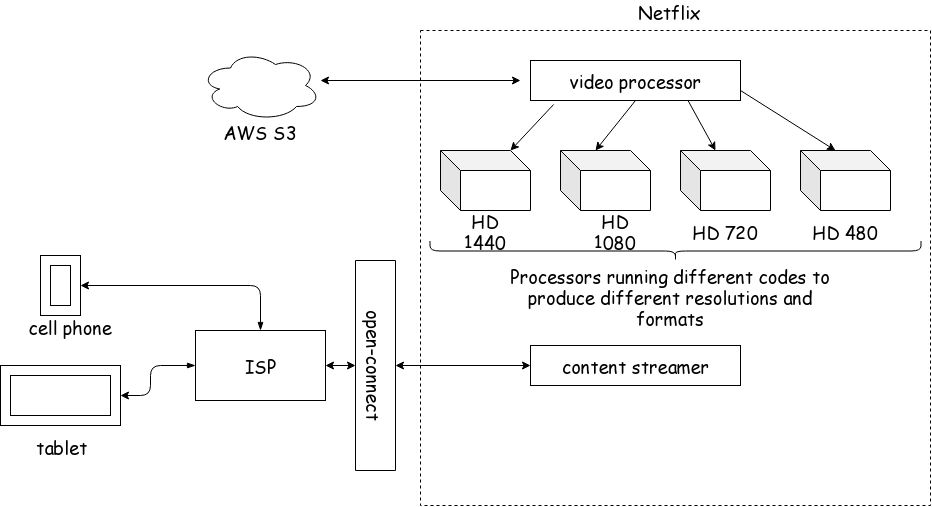
\includegraphics[width=13cm,height=10cm,keepaspectratio]{../media/crawler/netflix.png}
    \caption{Functional Partitioning in Netflix as an example}
    \label{fig:netflix}
  \end{figure}
Figure \ref{fig:netflix} shows how a netflix streaming service is divided into two major subsystems -
the video processor and the content streamer. This brings a lot of benefits but also increasing
engineering challenges. The main benefits are both service operate independently, parallel teams work
on independent codebases. Each service scales independently of other.
\item \textbf{Data partitioning}: Refers to maintaining subset of data onto each machine and controlling
  its state independent of other machines. This is the application of shared-nothing principle. With no
  data sharing, there is no data synchronization, no need for locking on global data store, and so
  failures can be isolated because nodes are not dependent on each other. A simplistic approach of data
  partitioning is distributing objects among machines based on first english alphabets of lookup key
  which maps to actual machine. A more sophisticated technique will use consistent hashing to partition
  subset of data fairly among machines and keeps distribution fair when capacity is increased/decreased.
  Hence, data when partition correctly, provides endless scalability - adding more users, handle more
  parallel connections, collecting more data and deploy program onto more servers.
\end{itemize}

\pagebreak

\subsection{Managing State}\label{managestate}
Managing state is often overlooked aspect when addressing the scaling problem of the application. If not done properly, it can create barriers to scale the application well. In a program environment where identical copies are used to perform some
computation, nodes using its own local/in-memory to cache objects are extremely
difficult/tricky to coordinate cache invalidation. In such cases, it is best to
maintain a global shared cache store so there is only one copy of each object and
easier to invalidate.
\begin{figure}[h!]
  \centering
  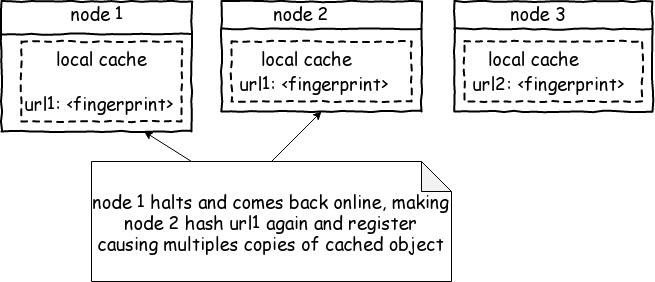
\includegraphics[width=10cm,height=8cm,keepaspectratio]{../media/crawler/multi-cache-wrng.png}
  \caption{redundant copes of same cached object}
  \label{fig:wrngcache}
\end{figure}
\\
\\
\noindent
Once you have a shared resource such as shared cache, for accessing them, locks are used to prevent race conditions and to synchronize access to shared resources. To achieve Horizontal Scalability(HS), distributed locks systems such as zookeeper \cite{zookeeper} or chubby \cite{chubby} can be considered. Many apps use local locks which causes bottlenecks. Instead of trying to share locks on web servers, you
should push the state out of applns servers similar to http session data store.
\begin{figure}[h!]
  \centering
  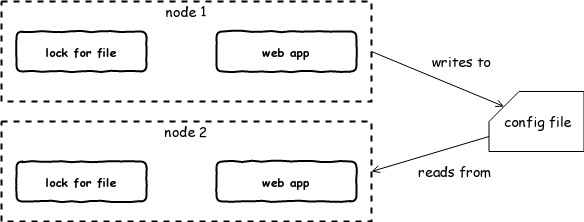
\includegraphics[width=10cm,height=8cm,keepaspectratio]{../media/crawler/wrng-local-locks.png}
  \caption{local locks preventing HS}
  \label{fig:wrnglocks}
\end{figure}
\\
\\
\noindent
To prevent the condition shown in figure \ref{fig:wrnglocks}, rule of thumb is to
use a combination of functional partitioning and scaling out using clones. Remove
the locking functionality from the application code and create an independent
service from it. Then lets the program clones use shared lock service to share
locks globally.

\pagebreak

\begin{figure}[h!]
  \centering
  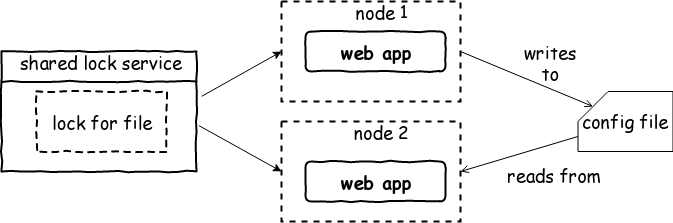
\includegraphics[width=13cm,height=10cm,keepaspectratio]{../media/crawler/rght-shared-locks.png}
  \caption{clones using shared locking mechanism}
  \label{fig:rghtlocks}
\end{figure}
\\
\\
\noindent
Potential disadvantage to using shared lock management is the increased latency.
Locks can be easily implemented with memcached/redis but not as robust as Zookeeper,
as it offers useful functionality for example - receiving notifications when a
lock gets released.